\subsection{Anemometer}
\begin{minipage}{0.55\textwidth}
Für die Windgeschwindigkeitsmessung wurde ein Ersatz Anemometer von Froggit genommen (Abb. \ref{fig:anemometer}). Das Anschlusskabel hat einen vier poligen RJ-11 Stecker, dessen Signal über eine Buchse zum MCU geführt wird. Das Anemometer selbst hat allerdings nur zwei Anschlüsse, die Speisung (rot) und das durch einen mit einem Dauermagneten schließbaren Reedkontakt modulierte pulsförmige Ausgangssignal (grün, Abb. \ref{fig:rj11stecker}). In der Abb. \ref{fig:beschaltungAnemometer} ist ersichtlich, dass das Ausgangssignal über R1 abfällt und C1 als Spannungsstabilisierung dient. Das daraus resultierende Signal ist in der Abb. \ref{fig:rechteckpuls_anemometer} aufgezeigt. Die Windgeschwindigkeit ist nun aus der Anzahl Rechteckpulsen direkt interpretierbar:\\

\end{minipage}
\begin{minipage}{0.44\textwidth}
\centering
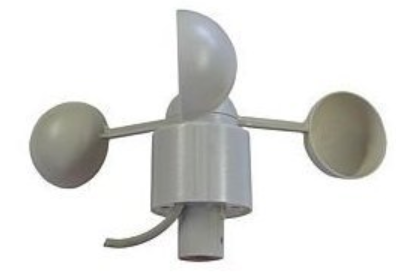
\includegraphics[width=0.9\textwidth]{graphics/Anemometer/anemometer.png}
\captionof{figure}{Anemometer \cite{AmazonAnemometer}}
\label{fig:anemometer}
\vspace{0.5cm}
\end{minipage}
\begin{minipage}{0.55\textwidth}
Wenn über einen Zeitraum $T$ die Anzahl Pulse $A$ gemessen werden, dann kann auf die Winkelgeschwindigkeit $\omega$ nach 
\begin{equation}
\centering
\omega=\frac{A}{T}\qquad[s^{-1}]
\end{equation}
geschlossen werden. Da allerdings verschiedene Faktoren wie das Trägheitsmoment des Schalenkreuzes, Reibungsverluste bei der Drehbewegung, Verfälschung bei wechselnder Windrichtung usw. zusätzlich auf das Anemometer wirken, wird es sehr komplex die Windgeschwindigkeit exakt zu berechnen. Deshalb wird nur ein Näherungswert ermittelt und mit einem Skalierungsfaktor $SF$ korrigiert. Somit ergibt sich für die Windgeschwindigkeit $v_{Wind}$ mit Radius $r$ des Schalenkreuzes
\begin{equation}
\centering
v_{Wind} = \frac{A*r*SF}{T}\qquad[m/s].
\label{equ:berechnungWindgeschwindigkeit}
\end{equation}
Der Skalierungsfaktor $SF$ wird mittels Referenzmessungen der Windgeschwindigkeit eines digitalen Anemometers eruiert. 
\end{minipage}
\begin{minipage}{0.44\textwidth}
\vspace{0.5cm}
\centering
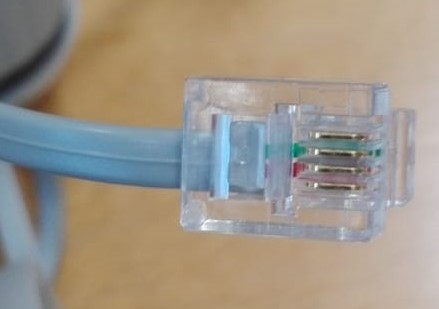
\includegraphics[width=0.9\textwidth]{graphics/Anemometer/rj_11_anschlussstecker.png}
\captionof{figure}{RJ-11 Stecker}
\label{fig:rj11stecker}
\vspace{0.5cm}
\end{minipage}
\begin{minipage}{0.55\textwidth}
\vspace{0.55cm}
\centering
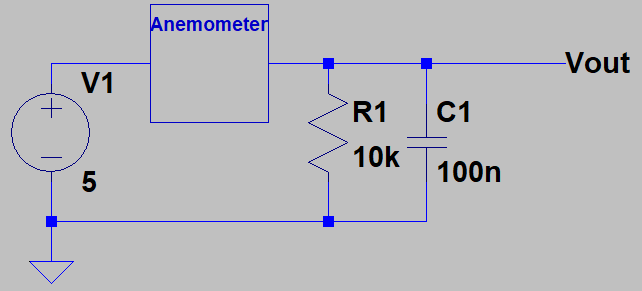
\includegraphics[width=\textwidth]{graphics/Anemometer/schaltung_anemometer.png}
\captionof{figure}{Beschaltung des Ausgangs des Anemometers.}
\label{fig:beschaltungAnemometer}
\end{minipage}
\begin{minipage}{0.44\textwidth}
\centering
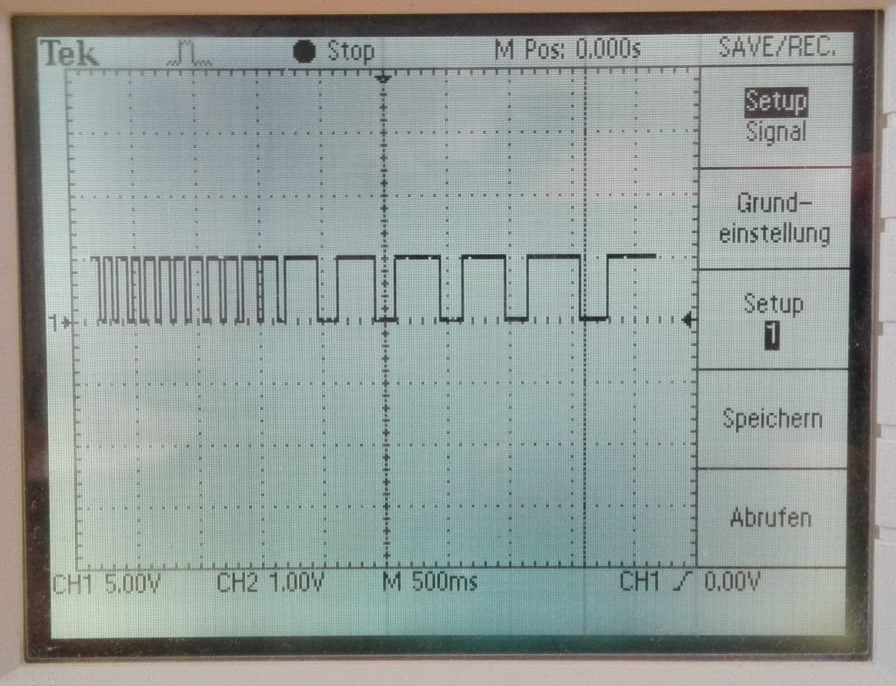
\includegraphics[width = 0.9\textwidth]{graphics/Anemometer/oszilloskop_anenometer_puls.png}
\captionof{figure}{Ausgangssignal $V_{out}$}
\label{fig:rechteckpuls_anemometer}
\end{minipage}
\newpage

\subsubsection{Implementation in die Firmware}
Die Implementation wurde recht simpel gehalten. Der gesamte implementierte Code für das Anemometer ist im Headerfile ''Anemometer.h'' extern deklariert und im File Anemometer.cpp initialisiert. Das Signal $V_{out}$ ist mit einen digital Pin des Atmega 2560 (Pinnummer 2 des Arduino Mega Boards) verbunden. Über einen Zeitraum von $5000ms$, auf die steigende Flanke getriggert, wird die Anzahl von Pulsen mittels Interrupt\footnote{es handelt sich hierbei um \textit{external Interrupts}.} gezählt. Dabei wird zuerst der Interrupt auf der Pinnummer 2 aktiviert, mit einem Delay von $5000ms$ gewartet, wobei bei jedem ausgelösten Interrupt die Funktion \textcolor{orange}{countWind}() ausgeführt und somit bei jeder steigenden Flanke um eins inkrementiert wird. Zum Schluss folgt die Deaktivierung des Interrupts und die Berechnung der Windgeschwindigkeit nach der Gleichung \ref{equ:berechnungWindgeschwindigkeit}.\\

\subsubsection{Validierung}
Über eine einigermaßen konstanten Windgeschwindigkeit eines Heizlüfters/Ventilators (mit verschiedenen Stärkestufen) wurden Messpunkte des Anemometers (Abb. \ref{fig:anemometer}), sowie auch des digitalen Anemometers (Abb. \ref{fig:digitalesAnemometer}) erfasst. In der Abb. \ref{fig:messpunkteAnemometer_Vergleich} sind diese Messwerte graphisch dargestellt.\\
\begin{minipage}{0.65\textwidth}
\vspace{0.5cm}
\centering

\includegraphics[width=\textwidth]{graphics/placeholder.png}
\captionof{figure}{Graph der Messwerte}
\label{fig:messpunkteAnemometer_Vergleich}
\end{minipage}
\begin{minipage}{0.34\textwidth}
\vspace{0.5cm}
\centering
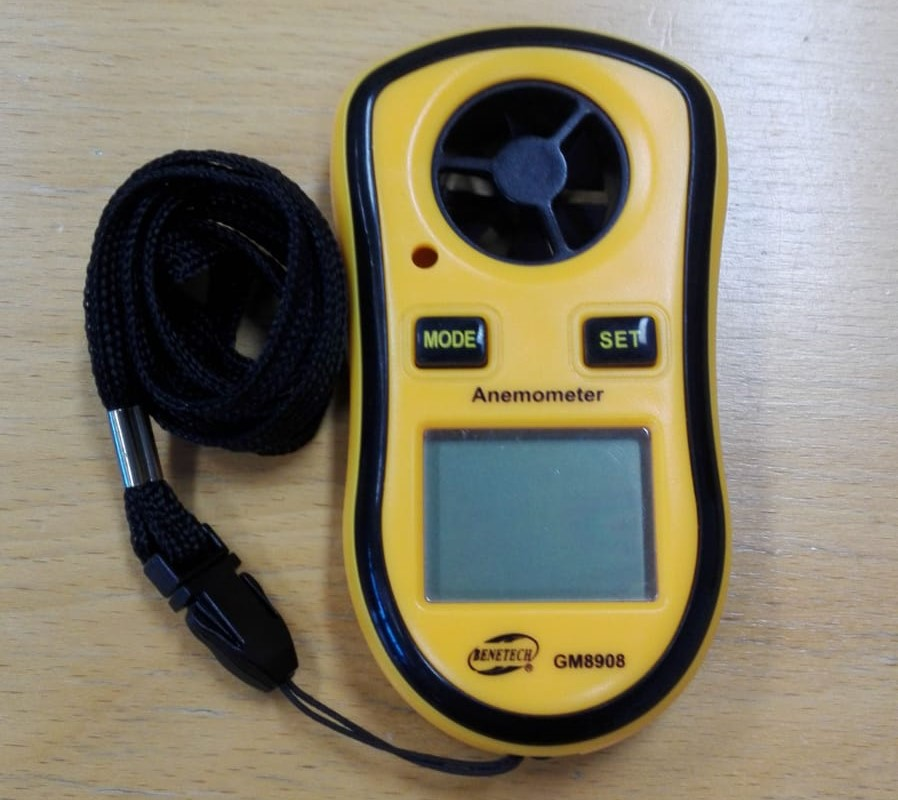
\includegraphics[width=\textwidth]{graphics/Anemometer/messgeraet_anemometer.png}
\captionof{figure}{Digitales Anemometer (Benetech GM8908) mit einer Auflösung von $0.1m/s$ und einer Unsicherheit von $\pm5\%$ \cite{digitalesAnemometerBenetech}}
\label{fig:digitalesAnemometer}
\end{minipage}
\todo[inline]{Hier muss noch die Interpretation der gemessenen Werte geschrieben werden.}
\newpage